\documentclass{article}

\usepackage{booktabs}
\usepackage{microtype}
\usepackage{pgfplots}
\usepackage{amsmath}

\title{Mandatory Assignment 2}
\author{Kris-Mikael Krister (krismikk)\\\texttt{krismikael@protonmail.com}}
\date{\today}

\begin{document}

\maketitle

\section*{Multilayer Perceptron}

The Multilayer Perceptron (MLP) is implemented with a fixed set of input and output nodes and one hidden layer. These are hyperparameters for the MLP and are constraints that won't change.

The network is trained using a subset of the available data, then verified using test data. The test data is a separated subset of the available data, and used to verify \emph{how well} the model performs. By using an earlystopping algorithm, the test data is used to avoid overfitting the model with the training data. By separating the test data from the training data, the earlystopping algorithm can help \emph{generalize} the resulting model. One run of the algorithm can be summarized as the following steps.

\begin{itemize}
    \item The available data is separated into training data, test data and validation data. The ratio is set to $50\%$, $25\%$ and $25\%$ of the total data respectively.
    \item Weights are randomly generated.
    \item One training round updates the weights a fixed number of iterations, set to $100$.
    \item After training, the model is verified using the \emph{validation data}. An error value is calculated.
    \item Training/verifidation repeats until the error value stops decreasing (earlystopping).
    \item The model is tested using the \emph{test data} and a confusion matrix is generated. The confusion matrix includes the percentage of correct values.
\end{itemize}

\noindent The amount of nodes/neurons in the hidden layer is a hyperparameter just as the number of input/ouput nodes. T amount can be tuned to generate the best model, which is in contrast to the other fixed hyperparameters. I chose to find the number by trial and error.

Initial weights are randomly generated in the algorithm, so the algorithm should run multiple times and the \emph{score} for each hidden node is calculated from the mean of the results\footnote{The algorithm written to solve the current problem runs fast enough to run multiple times and get the mean result. Note that such an approach could be impractical in other cases where the algorithm runs slower.}. The graph below shows the percentage of correct values for each tenth hidden node from $1 - 300$ ($n$ where $(n + 1) \mod{10} = 0$). The mean is calculated from 5 runs, where one run is explained in the above list.\\\\

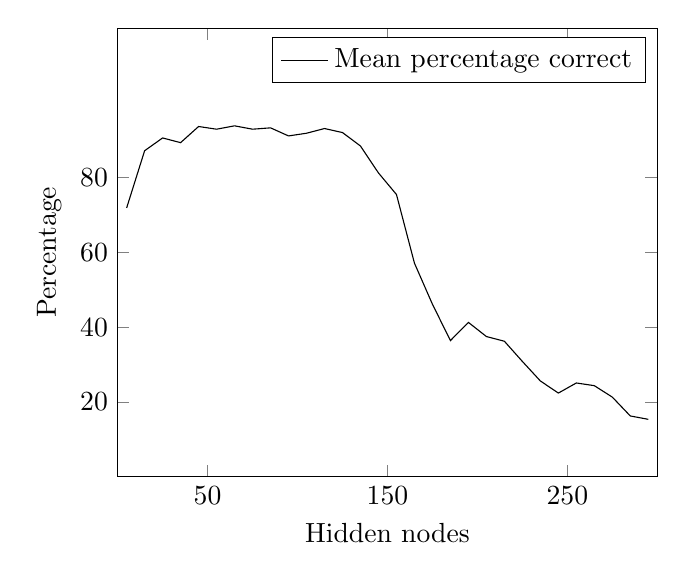
\begin{tikzpicture}
\begin{axis}[
    xlabel={Hidden nodes},
    ylabel={Percentage},
    xmin=0, xmax=300,
    ymin=0, ymax=120,
    xtick={50,150,250},
    ytick={20,40,60,80}
]
\addplot[
]
coordinates {
    (5,71.8918918919)(15,87.2072072072)(25,90.6306306306)(35,89.3693693694)(45,93.6936936937)(55,92.972972973)(65,93.8738738739)(75,92.972972973)(85,93.3333333333)(95,91.1711711712)(105,91.8918918919)(115,93.1531531532)(125,92.0720720721)(135,88.4684684685)(145,81.2612612613)(155,75.4954954955)(165,57.1171171171)(175,46.1261261261)(185,36.3963963964)(195,41.2612612613)(205,37.4774774775)(215,36.2162162162)(225,30.8108108108)(235,25.5855855856)(245,22.3423423423)(255,25.045045045)(265,24.3243243243)(275,21.2612612613)(285,16.2162162162)(295,15.3153153153)
};
\legend{Mean percentage correct}
\end{axis}
\end{tikzpicture}

\noindent These results indicate convergance to a maximum for just a few hidden nodes. Another interesting find is that around 150 hidden nodes the results drops significantly. For these two reasons, I will go more into detail for the nodes $5 - 30$. I will check each node, and increase the number of runs for each node to $50$. The mean is calculated and shown in the graph below.\\\\

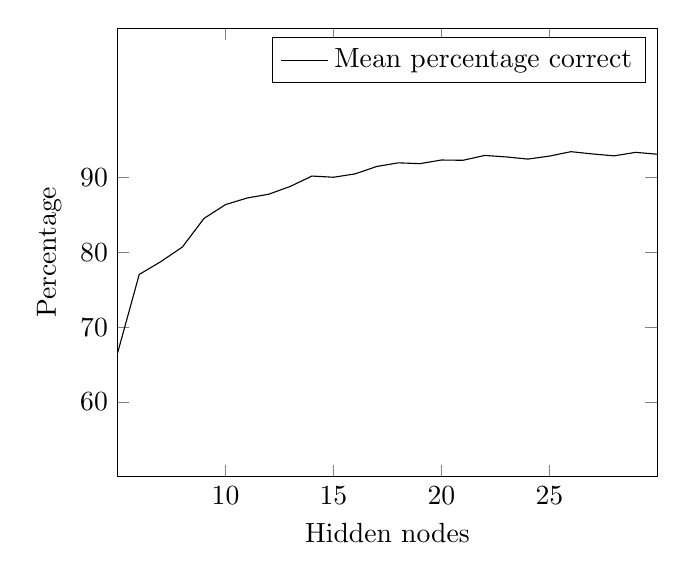
\begin{tikzpicture}
\begin{axis}[
    xlabel={Hidden nodes},
    ylabel={Percentage},
    xmin=5, xmax=30,
    ymin=50, ymax=110,
    xtick={10,15,20,25},
    ytick={60,70,80,90}
]
\addplot[
]
coordinates {
    (5,66.5585585586)(6,77.045045045)(7,78.7567567568)(8,80.7207207207)(9,84.5405405405)(10,86.3963963964)(11,87.2792792793)(12,87.7837837838)(13,88.8288288288)(14,90.2162162162)(15,90.0540540541)(16,90.5045045045)(17,91.4954954955)(18,91.981981982)(19,91.8738738739)(20,92.3603603604)(21,92.3243243243)(22,92.972972973)(23,92.7747747748)(24,92.4864864865)(25,92.8828828829)(26,93.4774774775)(27,93.1711711712)(28,92.9189189189)(29,93.3873873874)(30,93.1351351351)
};
\legend{Mean percentage correct}
\end{axis}
\end{tikzpicture}

\noindent For $14$ hidden nodes, the mean percentage correct is $90.2\%$. The number converges to $\approx 92\%$ for $18$ nodes. However, the running time increases when nodes are added so $14$ nodes is sufficient for this network to classify well. The table below shows results for even-numbered nodes.

\begin{center}
\begin{tabular}{cc}
\toprule
Hidden nodes & Mean percentage correct \\
\midrule
12 & $87.8$\\
14 & $90.2$\\
16 & $90.5$\\
18 & $92.0$\\
20 & $92.3$\\
22 & $92.3$\\
22 & $92.5$\\
24 & $92.5$\\
26 & $93.5$\\
28 & $92.9$\\
30 & $93.1$\\
\bottomrule
\end{tabular}
\end{center}

\subsection*{Confusion Matrix}

\noindent The confusion matrix for 14 nodes is shown below with $91.9\%$ correct classifications. Values on the diagonal are number of correctly classified instances, and values outside the diagonal are incorrectly classified instances. For example, Class 1 (the first row in the matrix) classifies incorrectly three times to Class 4, 5 and 6, respectively. Class 5 (the fifth row) is incorrectly classified two times for being Class 4.

\begin{itemize}
    \item Class 1 incorrectly classified to Class 4, 5 and 6.
    \item Class 5 incorrectly classified to Class 4.
    \item Class 7 incorrectly classified to Class 3 and 6.
    \item Class 8 incorrectly classified to Class 1 and 4.
\end{itemize}

\noindent Based on this matrix, it seems like the network has some issues with classifying Class 1, 4 and 6 correctly.

\begin{center}
\begin{verbatim}
[  8.   0.   0.   1.   1.   1.   0.   0.]
[  0.  17.   0.   0.   0.   0.   0.   0.]
[  0.   0.  19.   0.   0.   0.   0.   0.]
[  0.   0.   0.  12.   0.   0.   0.   0.]
[  0.   0.   0.   2.   9.   0.   0.   0.]
[  0.   0.   0.   0.   0.  11.   0.   0.]
[  0.   0.   1.   0.   0.   1.  12.   0.]
[  1.   0.   0.   1.   0.   0.   0.  14.]
\end{verbatim}
\end{center}

\end{document}
